
\section{Location diversity changes TE problem}
%Current TE model assumes a static traffc matrix but  application adaptation due to location diversity can change the traffic matrix based on congestion in network or even a change in routing in the network.
%\begin{figure}[htb]
%%\vspace{-0.3in}
% \begin{center}
%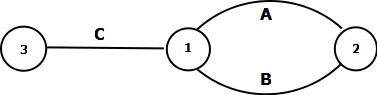
\includegraphics[scale=0.4]{final_images/Diagram3node.png}
%\end{center}
%	  \caption{Three Node Network}
%	\label{fig:3node} 
%%\vspace{0.1in}
%\end{figure}

% point: location diveristy makes TE difficult by changing TM; it is even difficult to estimate the traffic matrix after TE since 

The objective of TE is to ensure the the link utilization in the network is at minimal level but location can alter its effects by chanigng the traffic matrix and hence the utilization of links in the network.

\textbf{explain conditions}
We explain it using the three node netowrk in Figure~\ref{fig:3node}.
All link have capacity of 100 units and a constant delay.  Link A has a very small delay compared to links B and C; both B and C have equal delay. Node 1 has 100 units of demand which it can route from 2 as well as 3. In addition there is 20 units of demand at node 1 which it routes from 2. We assume that that the aggregate flow at a node constitutes of infinitesimal flows which can be split among multiple source locations. Similar to parallel TCP behavior, the ratio in which flows are split among multiple locations is inversely proportional to delay from a location. The routing in network is shortest path routing based on link weights and traffic is split equally among multiple path with equal weights.

\textbf{point: TE cannot be achieved since adaptation changes TM.}
Initially, link weights of A, B and C as 3, 2, 1 respectively. The traffic between 1 and 2 is routed only using B. 1 splits its demand of 100 units equally among 2 and 3. Thus traffic on links is A = 0, B = 70, and C = 50. In the next step, to balance load between A and B both link are set equal weights.  Let see how parallel TCP connections would change our estimates of link utilization in this case. Assuming each infinitesimal flow uses only one of the two links A and B, 50 unit of demand at 1 is routed using links B and C, and equal amount using A an C. In addition, the 20 units of background traffic is split equally among links B and C.  Since A has a much smaller delay than C, 50 units of demand at 1 routed using A and C will flow entirely through A. The demand routed using B and C will be split equally among B and C respectively. Thus traffic on links is A = 60, B = 35, and C = 25 which is different from expected values of A = 35, B = 35, C = 50. Thus, location diversity makes TE difficult by changing the traffic matrix and changing expected link utilization.
